\chapter{Results}
\label{chapter:Results}

\begin{introduction}
    "The only source of knowledge is experience." - Albert Einstein
\end{introduction}

\section{Evolution of Software Development}

The software development process has undergone several important stages, each enhancing its functionality and usability. The figures below illustrate the application's progress, showcasing different phases of refinement as the project matured.

\subsection{Initial Stages: Basic Functionality and User Interaction}

The first figure (Figure \ref{fig:v1}) represents the early stages of development, where the primary focus was on creating a user-friendly interface for calculating Average Read Depth and Depth of Coverage at diferent threshold from a \ac{bam} file for a Single Gene. In this version, the application prominently features a two-step process where the user selects a \ac{bed} file releated to the gene to analyse and one or more \ac{bam} files. These files are then processed to calculate key metrics, which are displayed in a results table. This simple design allowed for efficient user interaction but was somewhat limited in terms of flexibility and scope.

At this stage, the core challenge was to ensure that the software could handle large genomic files while presenting the results in a clear and intuitive format. The layout emphasizes simplicity, making it easier for users to navigate through the two-step process. However, as the project progressed, the need for more advanced features became evident.

\begin{figure}[H]
    \centering
    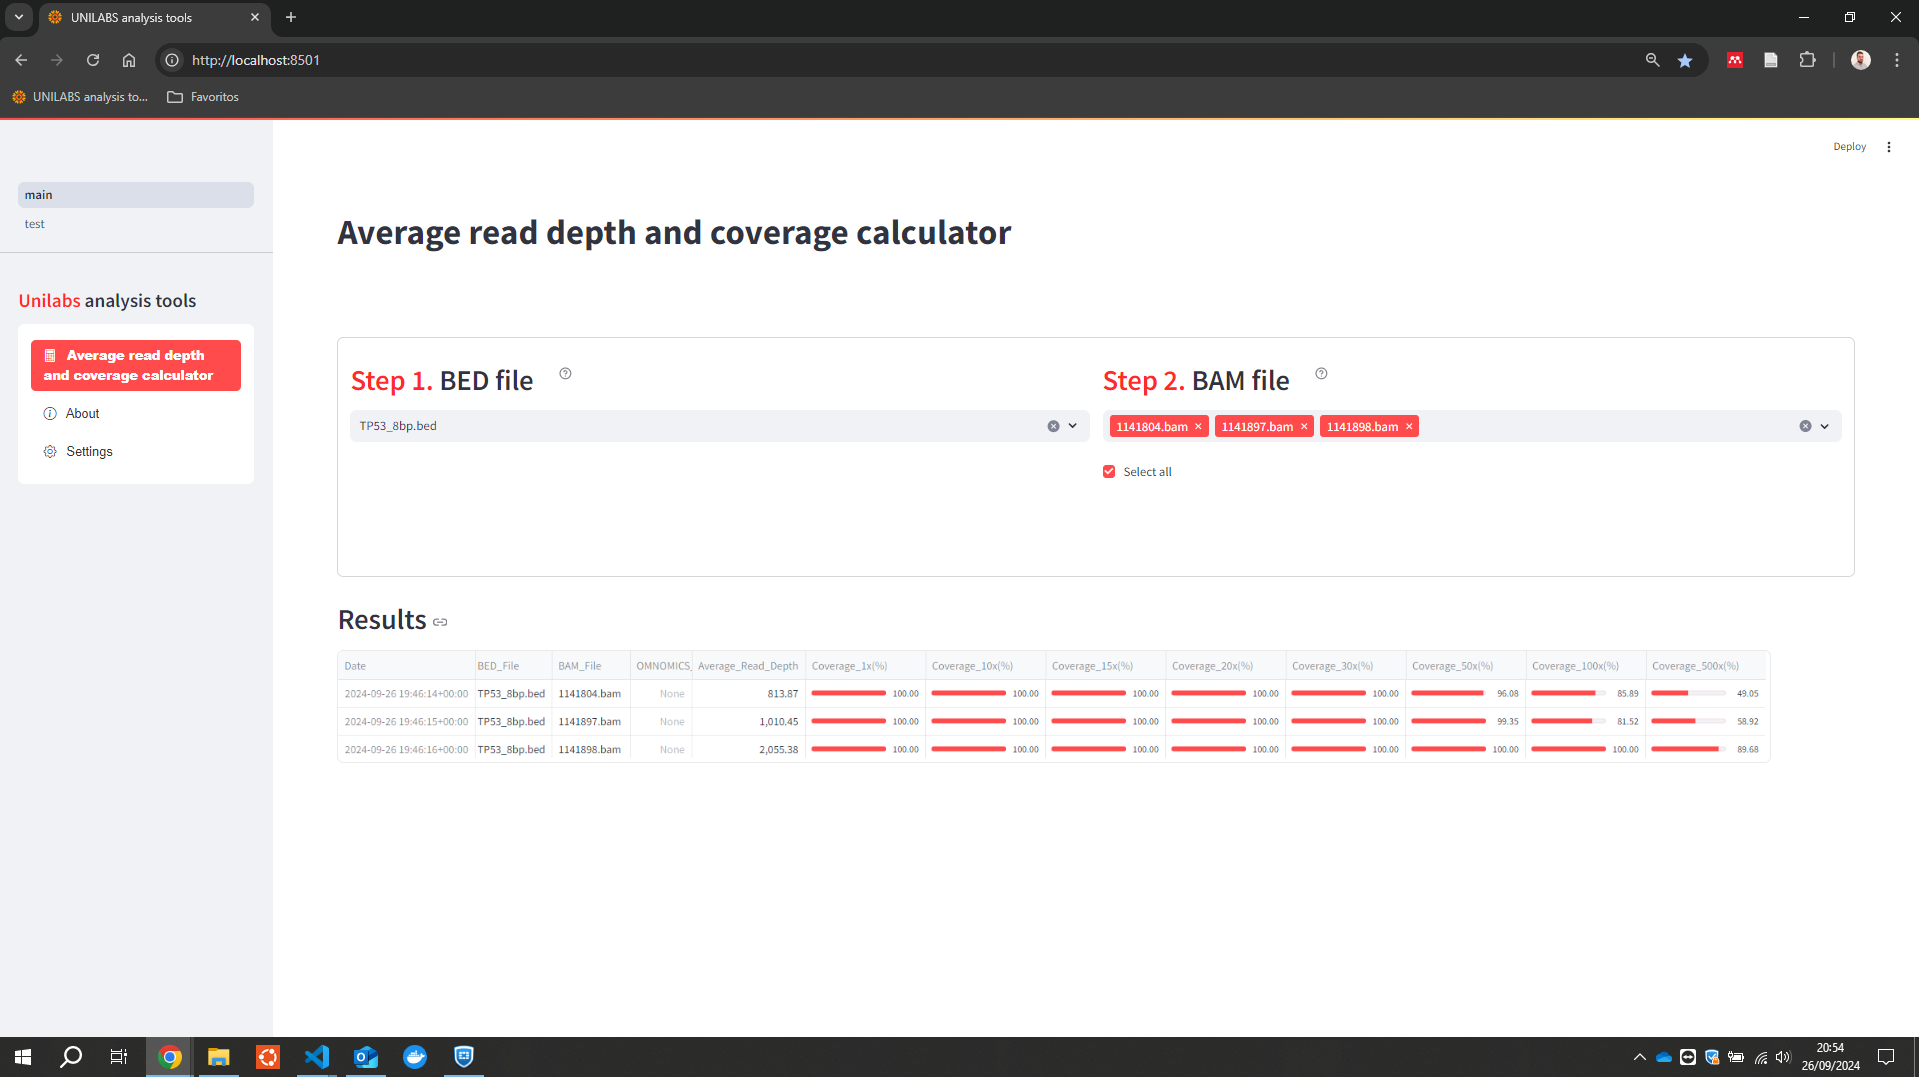
\includegraphics[width=1\textwidth]{figs/v1.png}
    \caption{First version of the \ac{gui}.} 
    \label{fig:v1}
\end{figure}

\subsection{Refinement: Introducing Flexibility and Multiple Analysis Modes}

In the second figure (Figure \ref{fig:v2}), the software has significantly evolved to include more detailed analysis options. The interface now presents multiple analysis types: \textit{Single Gene}, \textit{Gene Panel}, and \textit{Exome}, catering to different research needs. This flexibility represents a major shift from the earlier version, as it now allows users to select specific genome assemblies and regions of interest by using an Universal \ac{bed} file. Additionally, the results section has been split into tabs such as \textit{Overview} and \textit{Exon Details}, giving users the ability to drill down into the metrics for a the gene or explore exon-level coverage details. However, even though this last features were thinked to be used in this version, they only have been work fully in the last version of the software.

\begin{figure}[H]
    \centering
    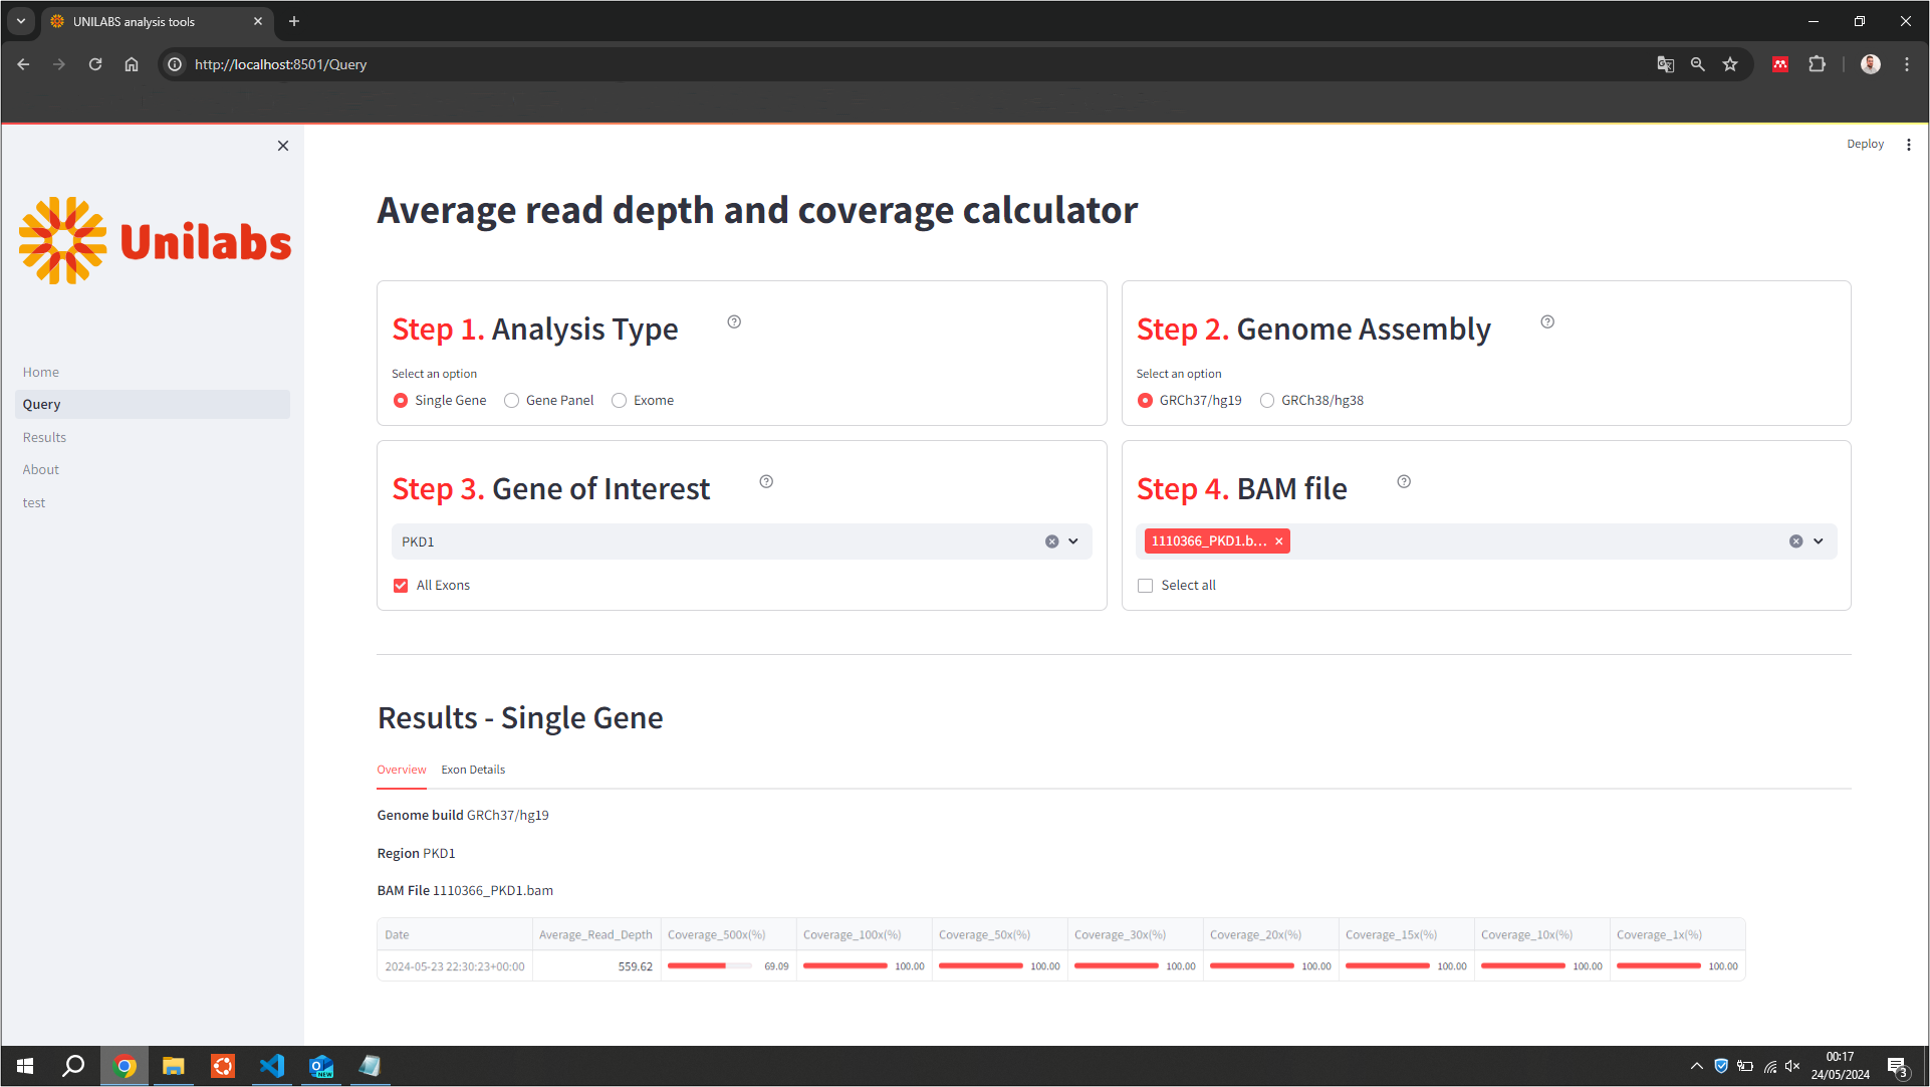
\includegraphics[width=1\textwidth]{figs/v2.png}
    \caption{Second version of the \ac{gui}.} 
    \label{fig:v2}
\end{figure}


The final version of the software is presented in the next section in detail with real-world data to showcase its full capabilities and effectiveness in genomic analysis. This final iteration represents the culmination of numerous improvements in both the user interface and the backend computational logic.

\subsection{Overview of the Final Version}

The final version of the software maintains the core functionality established in earlier versions, such as calculating Average Read Depth and Depth of Coverage from \ac{bed} and \ac{bam} files. However, it has evolved to include more refined features, enhanced performance, and the ability to handle more complex datasets.

This section presents a detailed overview of the final version of the software using real-world genomic data, illustrating its capabilities in calculating Depth and Breadth of Coverage for genomic regions of interest. The images provided demonstrate the final interface and processing stages.

\subsubsection{\textbf{Login Interface}}

As seen in Figure \ref{fig:login}, the software begins with a user authentication process, offering a simple and clean login interface. This feature, although optional in the final deployment, ensures that access to sensitive data is controlled. However, it is important to note that the current implementation of the login interface is a prototypical version and does not offer any form of security. The system does not perform encryption or validation of credentials beyond basic checks, and therefore it should not be relied upon for securing sensitive information. Further development would be required to implement a secure authentication system if needed in future deployments.

\begin{figure}[H]
    \centering
    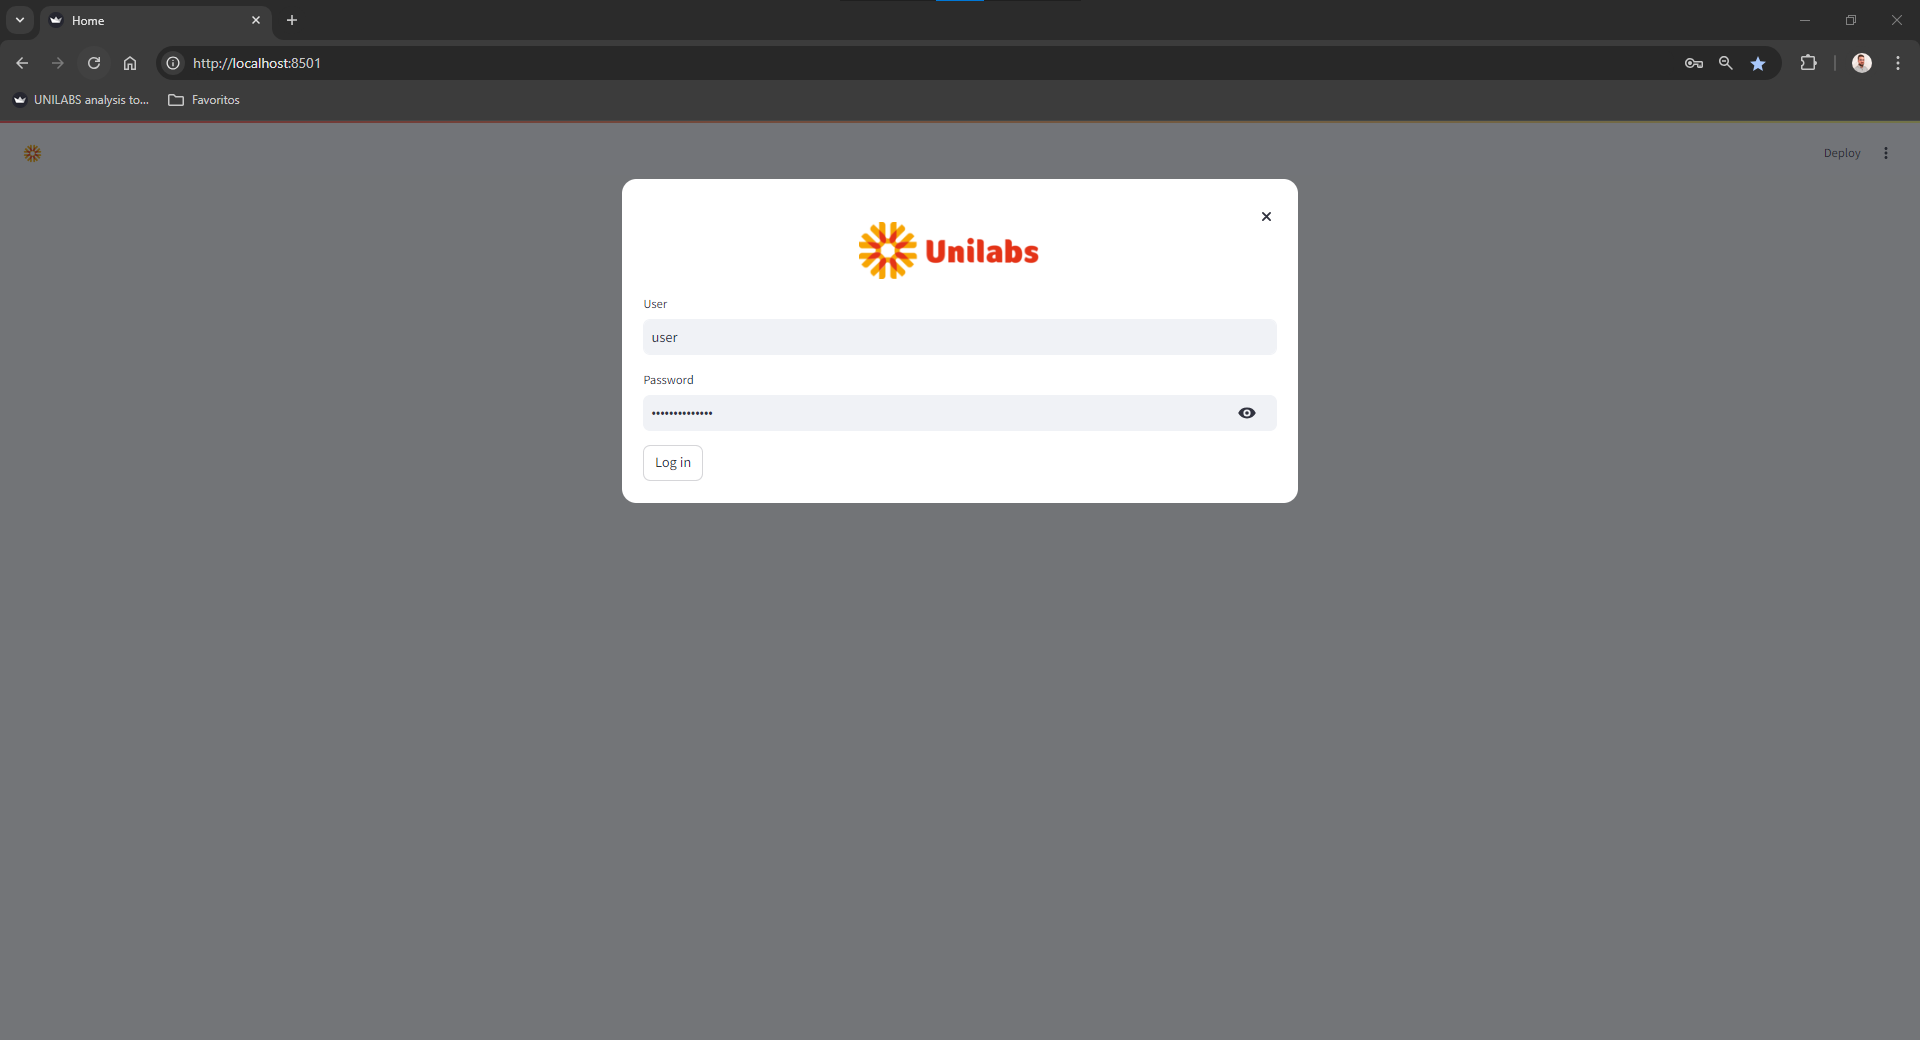
\includegraphics[width=\textwidth]{figs/v3.1.png}
    \caption{Login Interface for the Software}
    \label{fig:login}
\end{figure}

The next step of the process involves selecting the analysis type, as shown in Figure \ref{fig:single_gene}. Users can choose between three options: Single Gene, Gene Panel, and Exome. This selection determines the scope of the analysis and the subsequent steps in the workflow.


\subsubsection{\textbf{Single Gene Analysis}}

In this version, users can perform a single gene analysis by selecting the appropriate options for genome assembly and gene of interest. The software also provides the option to analyze all exons within the selected gene or focus on specific exons of interest. \ac{bam}/\ac{cram} files containing the sequencing data are acessed and processed by Samtools for detailed metrics.

\begin{figure}[H]
    \centering
    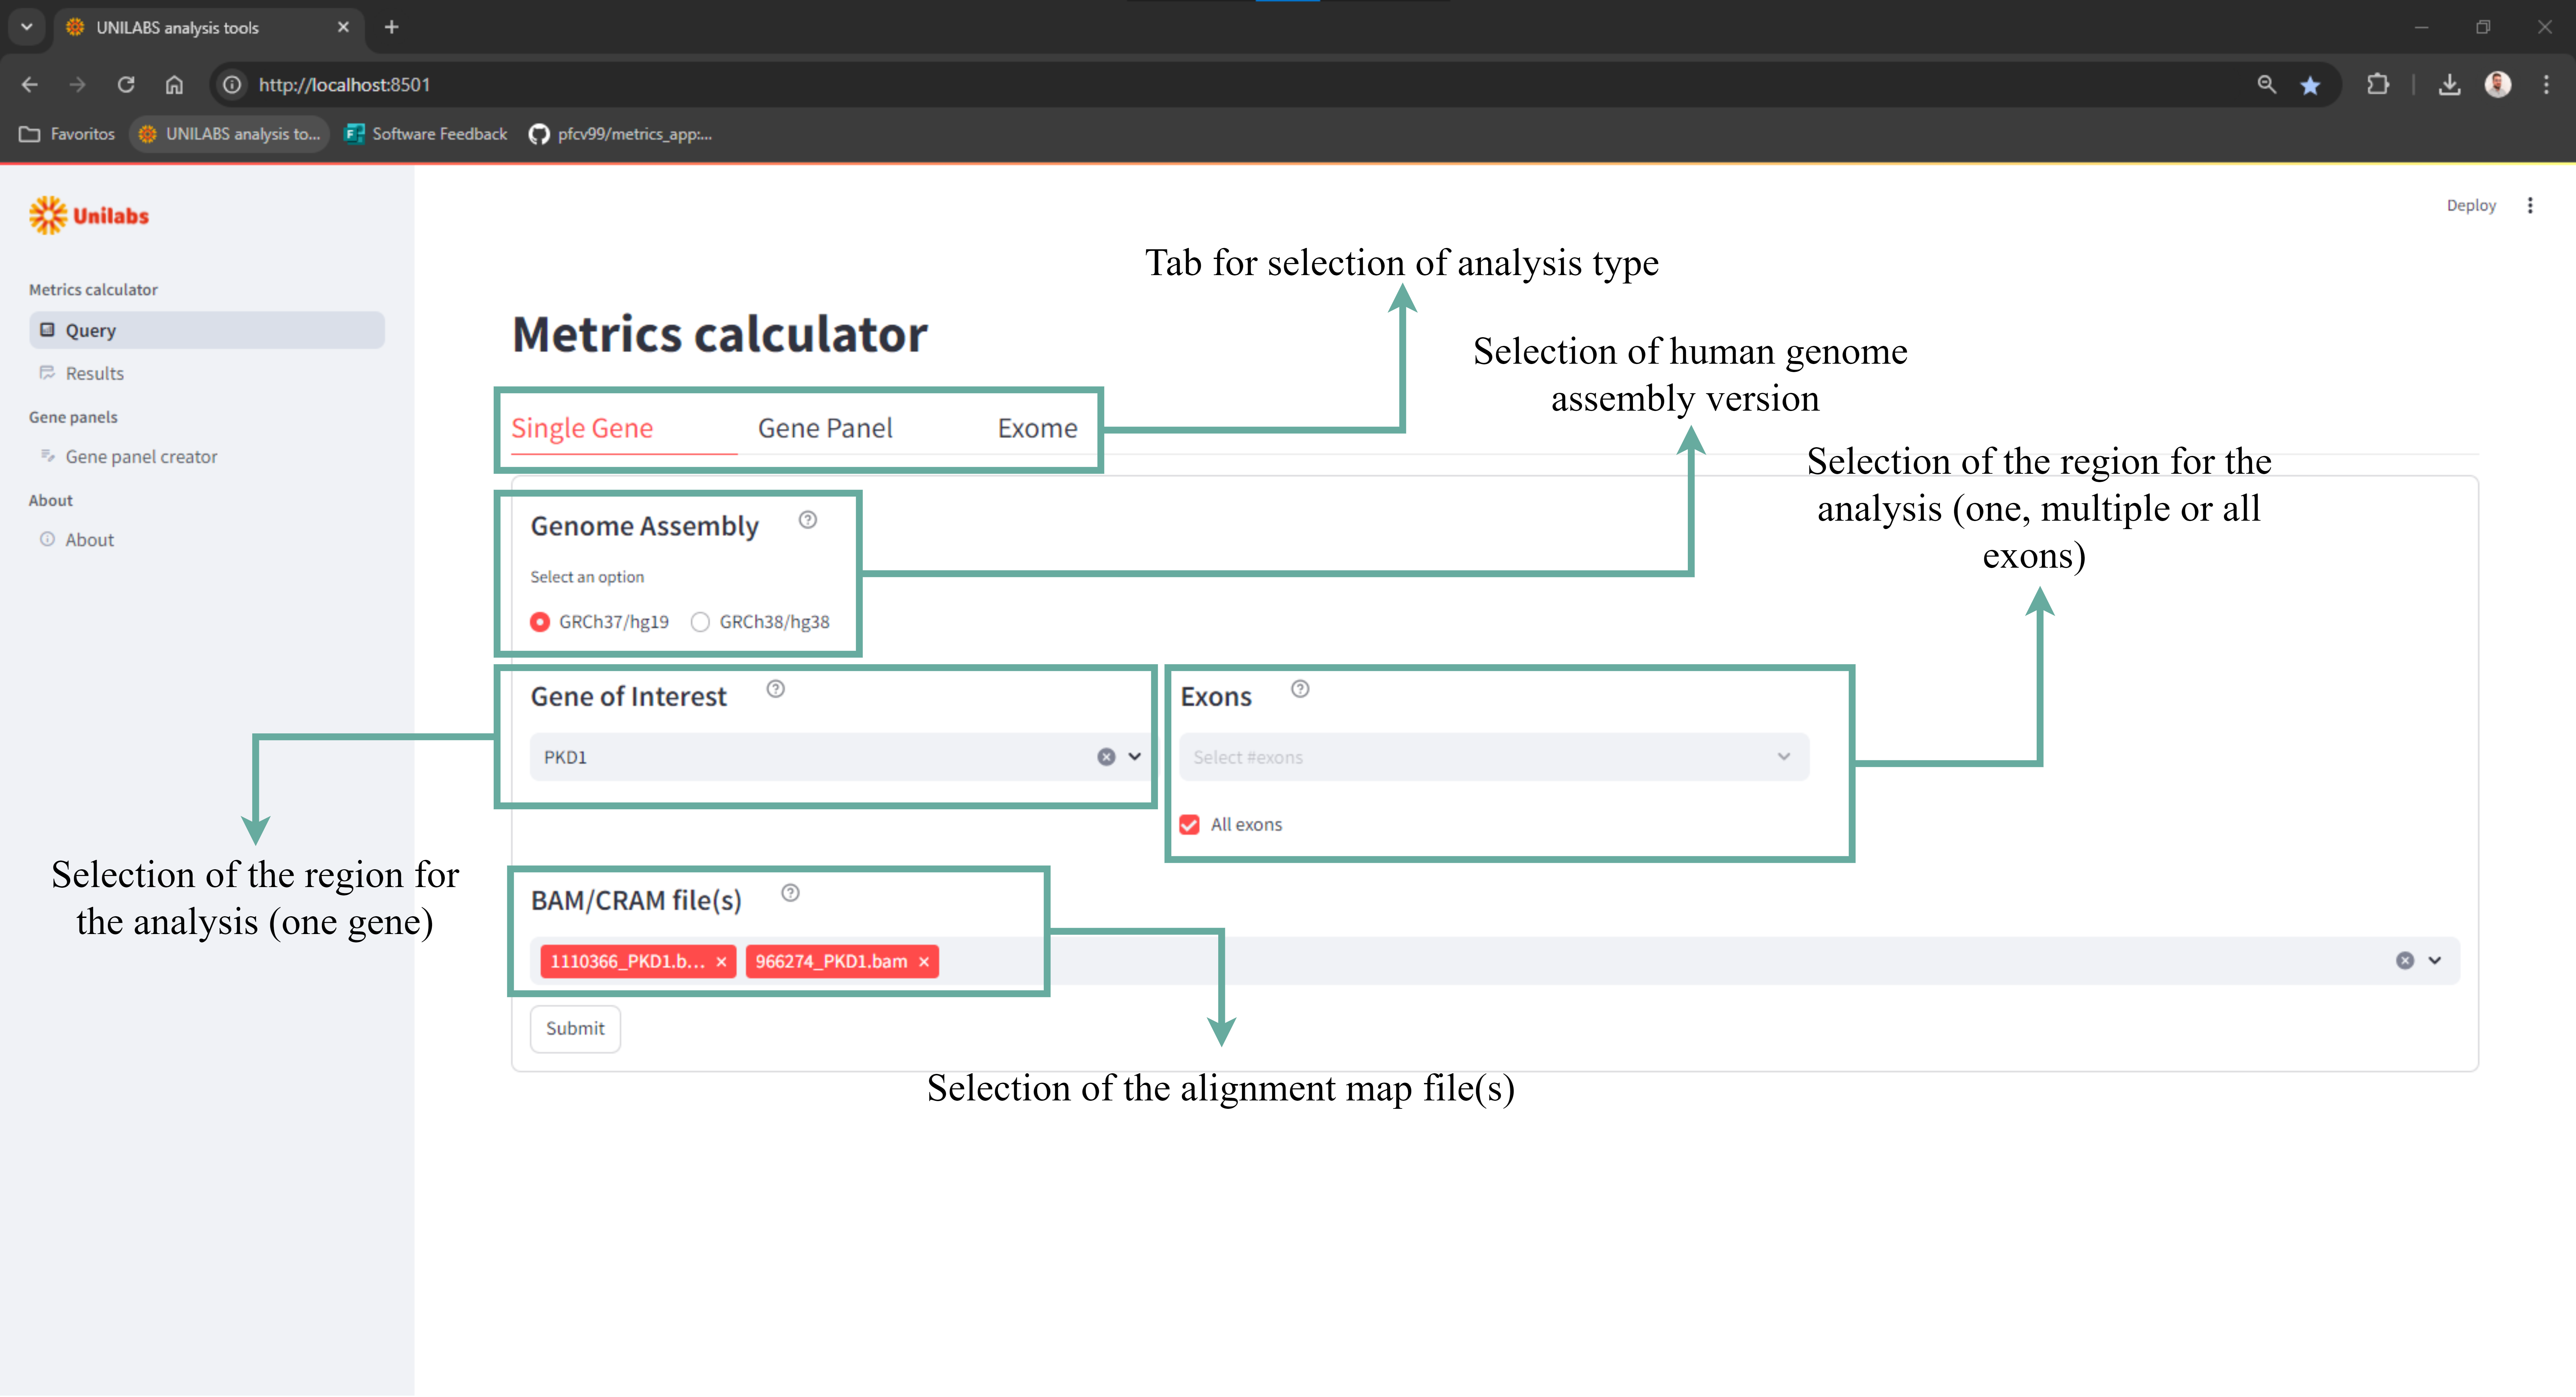
\includegraphics[width=\textwidth]{figs/v3.2.png}
    \caption{Single Gene Analysis Workflow}
    \label{fig:single_gene}
\end{figure}

\begin{itemize}
    \item \textbf{Results and Report Generation}

    Once the data is processed, users can access the results in the \texttt{Results} tab, as seen in Figure \ref{fig:results_loading}. The software compiles a detailed report that includes various metrics such as Average Read Depth, Breadth of Coverage, and Depth of Coverage percentages across different thresholds (e.g., 10x, 20x, 30x). This data is also available for download in a \ac{csv} or \ac{pdf} format, ensuring users can retain a permanent copy of the analysis results.
    
    \begin{figure}[H]
        \centering
        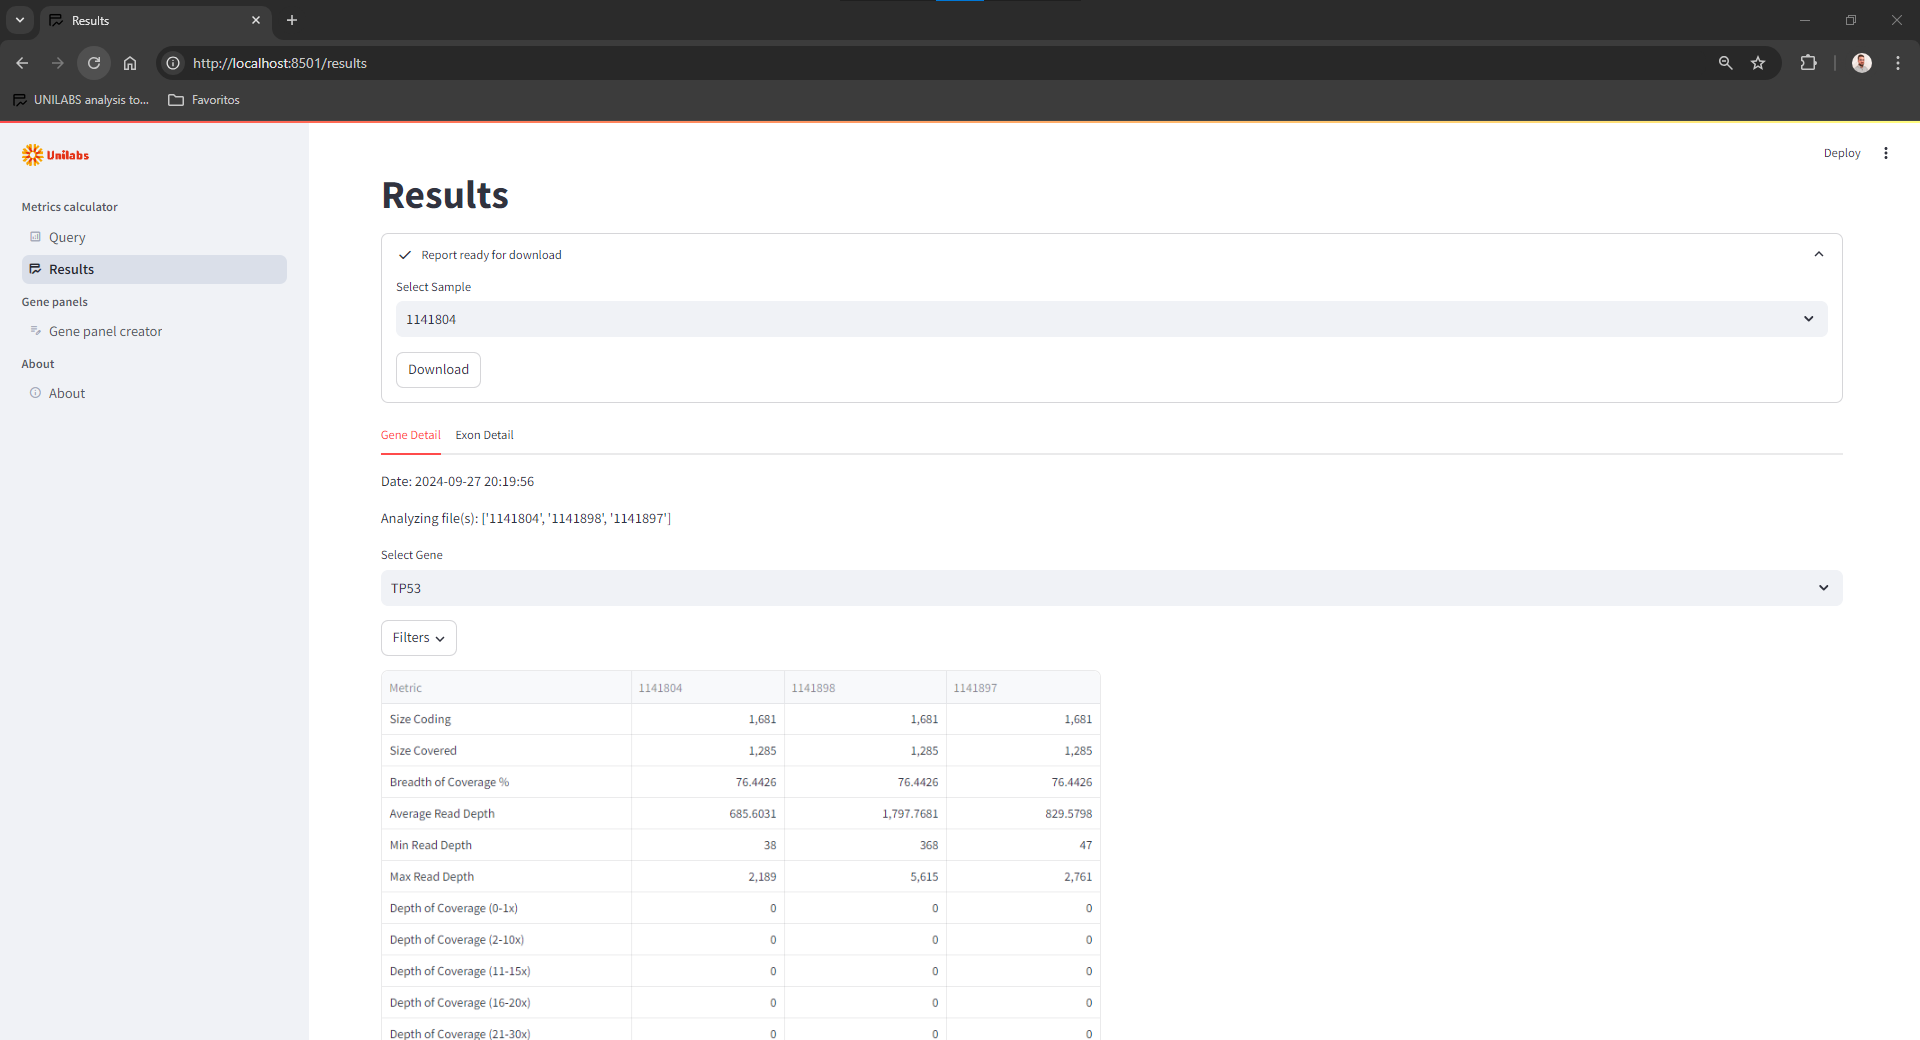
\includegraphics[width=\textwidth]{figs/v3.3.png}
        \caption{Results Tab Loading the Final Report}
        \label{fig:results_loading}
    \end{figure}
    
    In Figure \ref{fig:results_loading} and \ref{fig:final_report}, the detailed metrics for the gene \textit{TP53} are displayed, offering both gene-level and exon-level statistics. This comprehensive breakdown allows researchers to thoroughly assess the sequencing coverage for the analyzed samples. Key metrics include the Size Coding of the gene, minimum and Maximum Read Depth, and coverage percentages across various depth thresholds, providing valuable insights into the quality and completeness of the sequencing data.
    
    For this case study, the Size Coding of the \textit{TP53} gene is 1,681 \ac{bp}, with a Size Covered of 1,285 \ac{bp} for all three samples, resulting in a Breadth of Coverage of 76.4\%. The Average Read Depth across the three samples was 685.6x, 1,797.8x, and 829.6x, respectively. Depth of Coverage, or the number of times a particular region of the genome is covered by reads, directly impacts the reliability of variant detection, gene expression studies, and other genomic analyses. Inconsistent or insufficient depth may lead to variability in the ability to accurately detect mutations or copy number variations, potentially resulting in false positives or false negatives. For instance, lower depth may miss variants that are present at low frequencies, while higher depth ensures that even rare mutations are confidently identified. \cite{Larson2023}
    
    When examining the Depth of Coverage across different thresholds, the percentages for the 10x, 20x, and 30x thresholds were consistently 100\% for all three samples, demonstrating that all regions of interest achieved sufficient coverage at these lower thresholds. However, at higher thresholds, the Depth of Coverage showed more variability. For the 50x threshold, the coverage percentages were 95.3\%, 100\%, and 99.2\%, respectively. Similarly, at the 100x threshold, the coverage percentages were 83.8\%, 100\%, and 78.5\%. Finally, at the highest threshold of 500x, the coverage percentages dropped more significantly, with values of 41.4\%, 88.2\%, and 52.8\%, respectively.
    
    \begin{figure}[H]
        \centering
        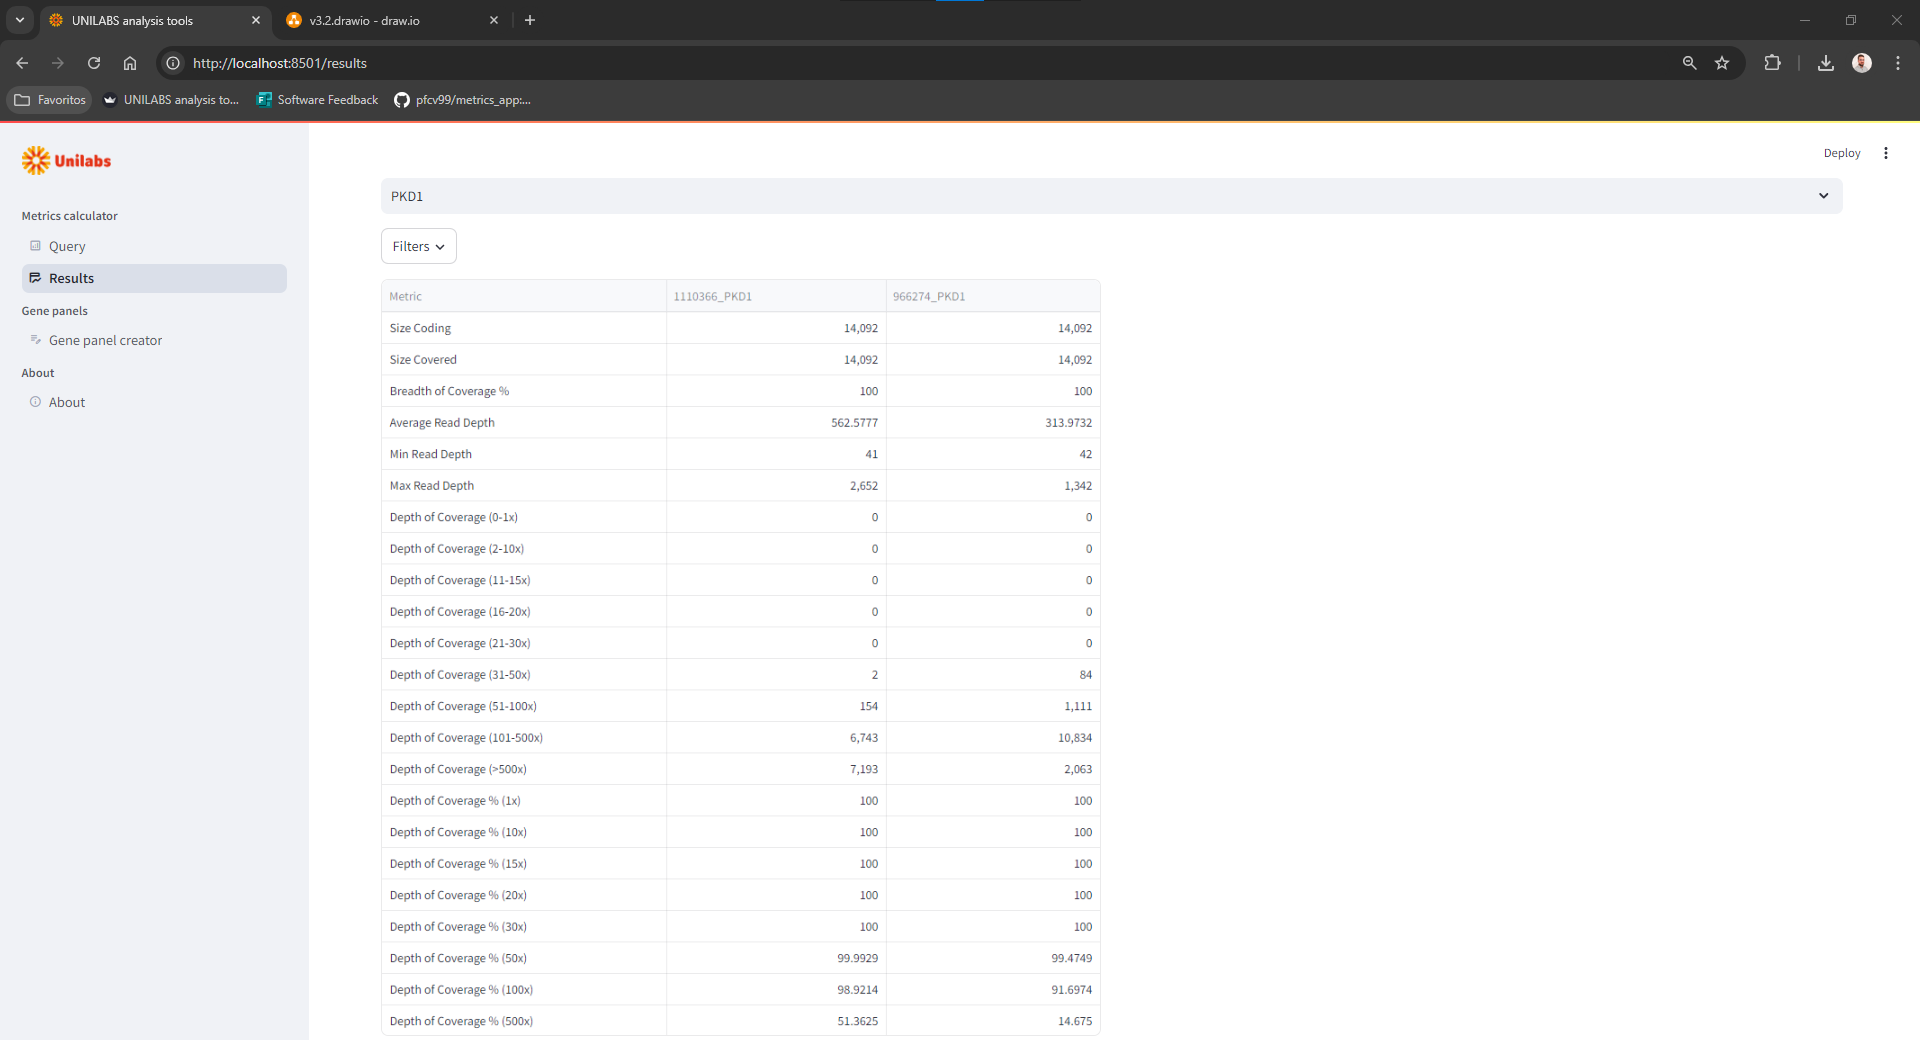
\includegraphics[width=\textwidth]{figs/v3.4.png}
        \caption{Final Report with Detailed Metrics for Gene TP53}
        \label{fig:final_report}
    \end{figure}
    
    \item \textbf{Depth of Coverage Visualization}
    
    One of the critical features of the final software version is its ability to visualize in a plot the distribution of Depth of Coverage across each position, as shown in Figure \ref{fig:coverage_plot}. This visualization allows users to see the depth of sequencing across the gene of interest, with blue regions highlighting exons. A threshold can be set by the user, and regions that fall below this threshold are highlighted in red, ensuring that gaps or low-coverage areas are easily identified. This is particularly important for researchers assessing the completeness of their sequencing data.
    
    \begin{figure}[H]
        \centering
        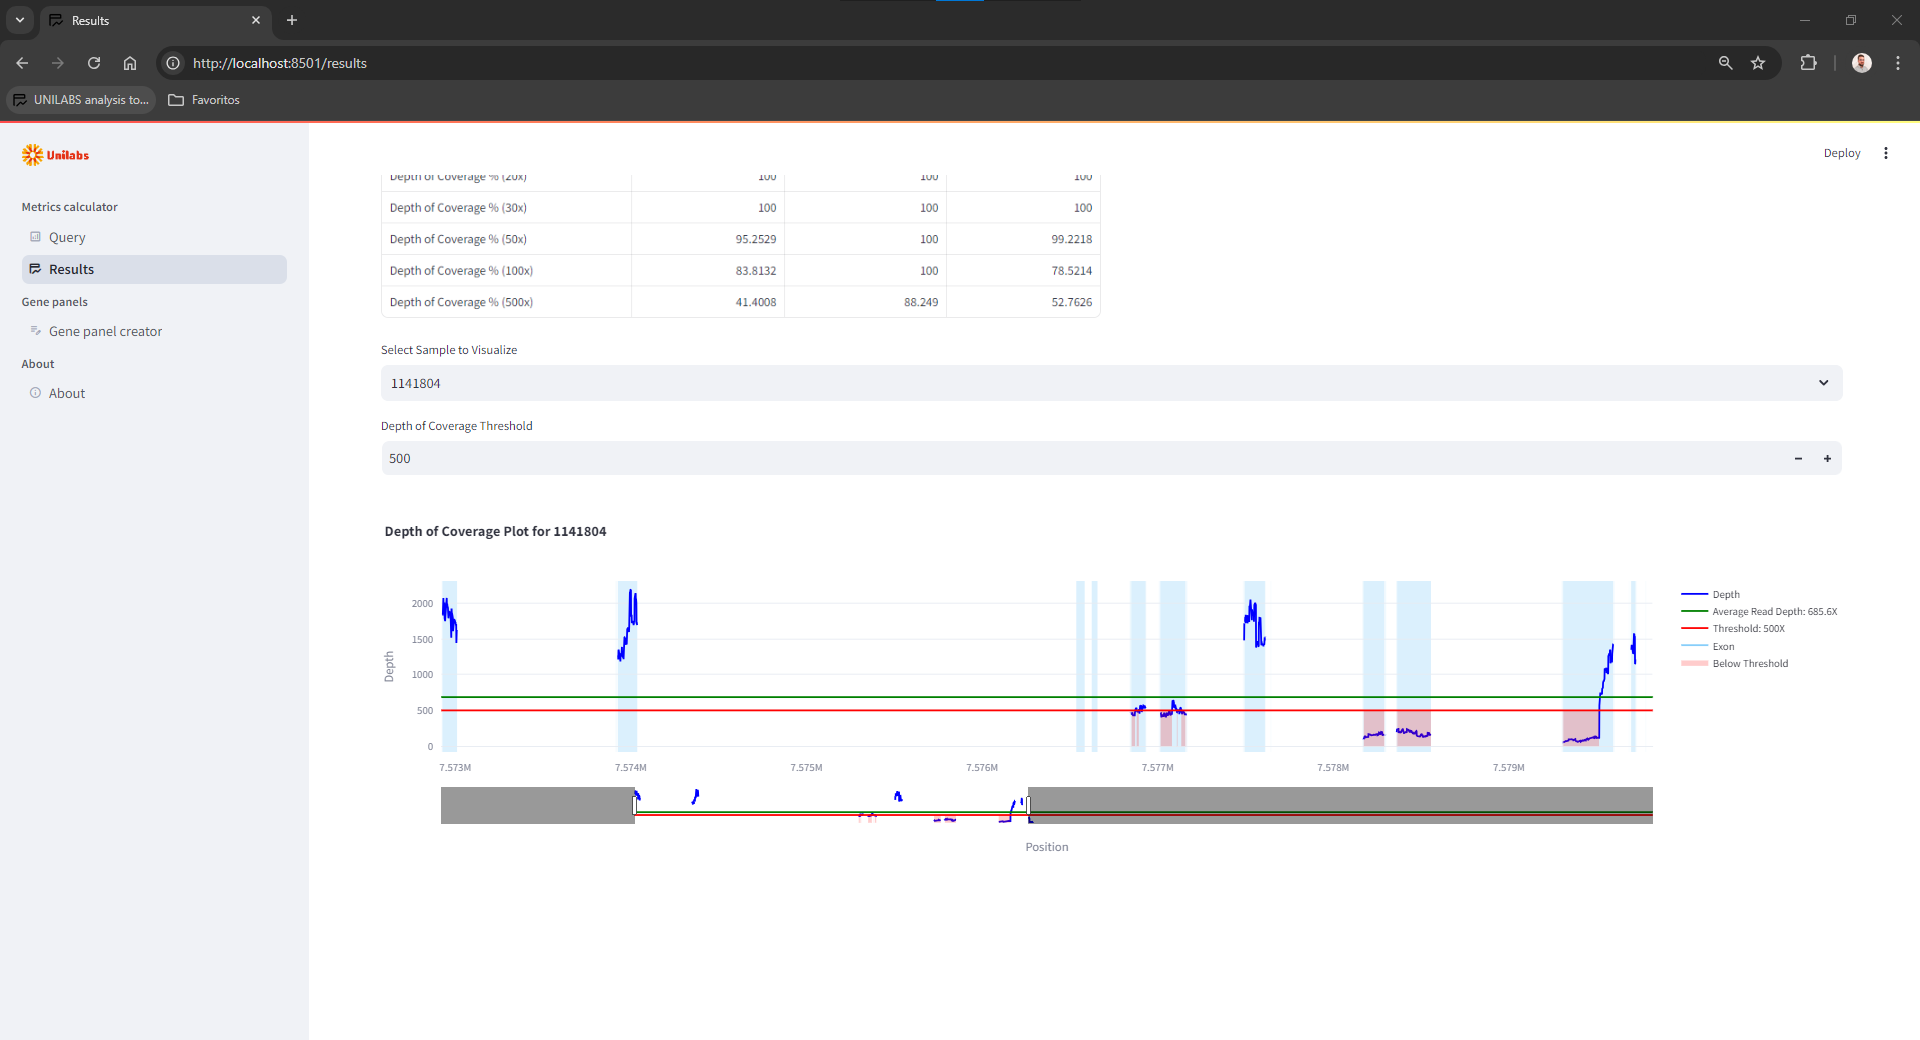
\includegraphics[width=\textwidth]{figs/v3.5.png}
        \caption{Depth of Coverage Visualization for Gene TP53}
        \label{fig:coverage_plot}
    \end{figure}
\end{itemize}

\subsubsection{\textbf{Gene Panel Analysis}}

In the gene panel analysis, the software is configured to process multiple genes simultaneously, as opposed to the single gene analysis. This functionality is particularly useful when studying gene panels associated with specific hereditary diseases, such as the BRCA1 and BRCA2 genes, commonly linked to breast and ovarian cancer. The analysis workflow is similar to that of a single gene but extends to multiple regions of interest, providing broader insights into the Depth and Breadth of Coverage across the entire panel.

\begin{itemize}
\item \textbf{Panel Selection and Input}

The user begins by selecting the appropriate genome assembly and the gene panel of interest. For this case study, the panel for breast and ovarian cancer was selected, which includes 27 genes, among which the BRCA1 and BRCA2 genes. The input consists of a \ac{bam} or \ac{cram} file associated with the selected panel, as shown in Figure \ref{fig:panel_input}.

\begin{figure}[H]
    \centering
    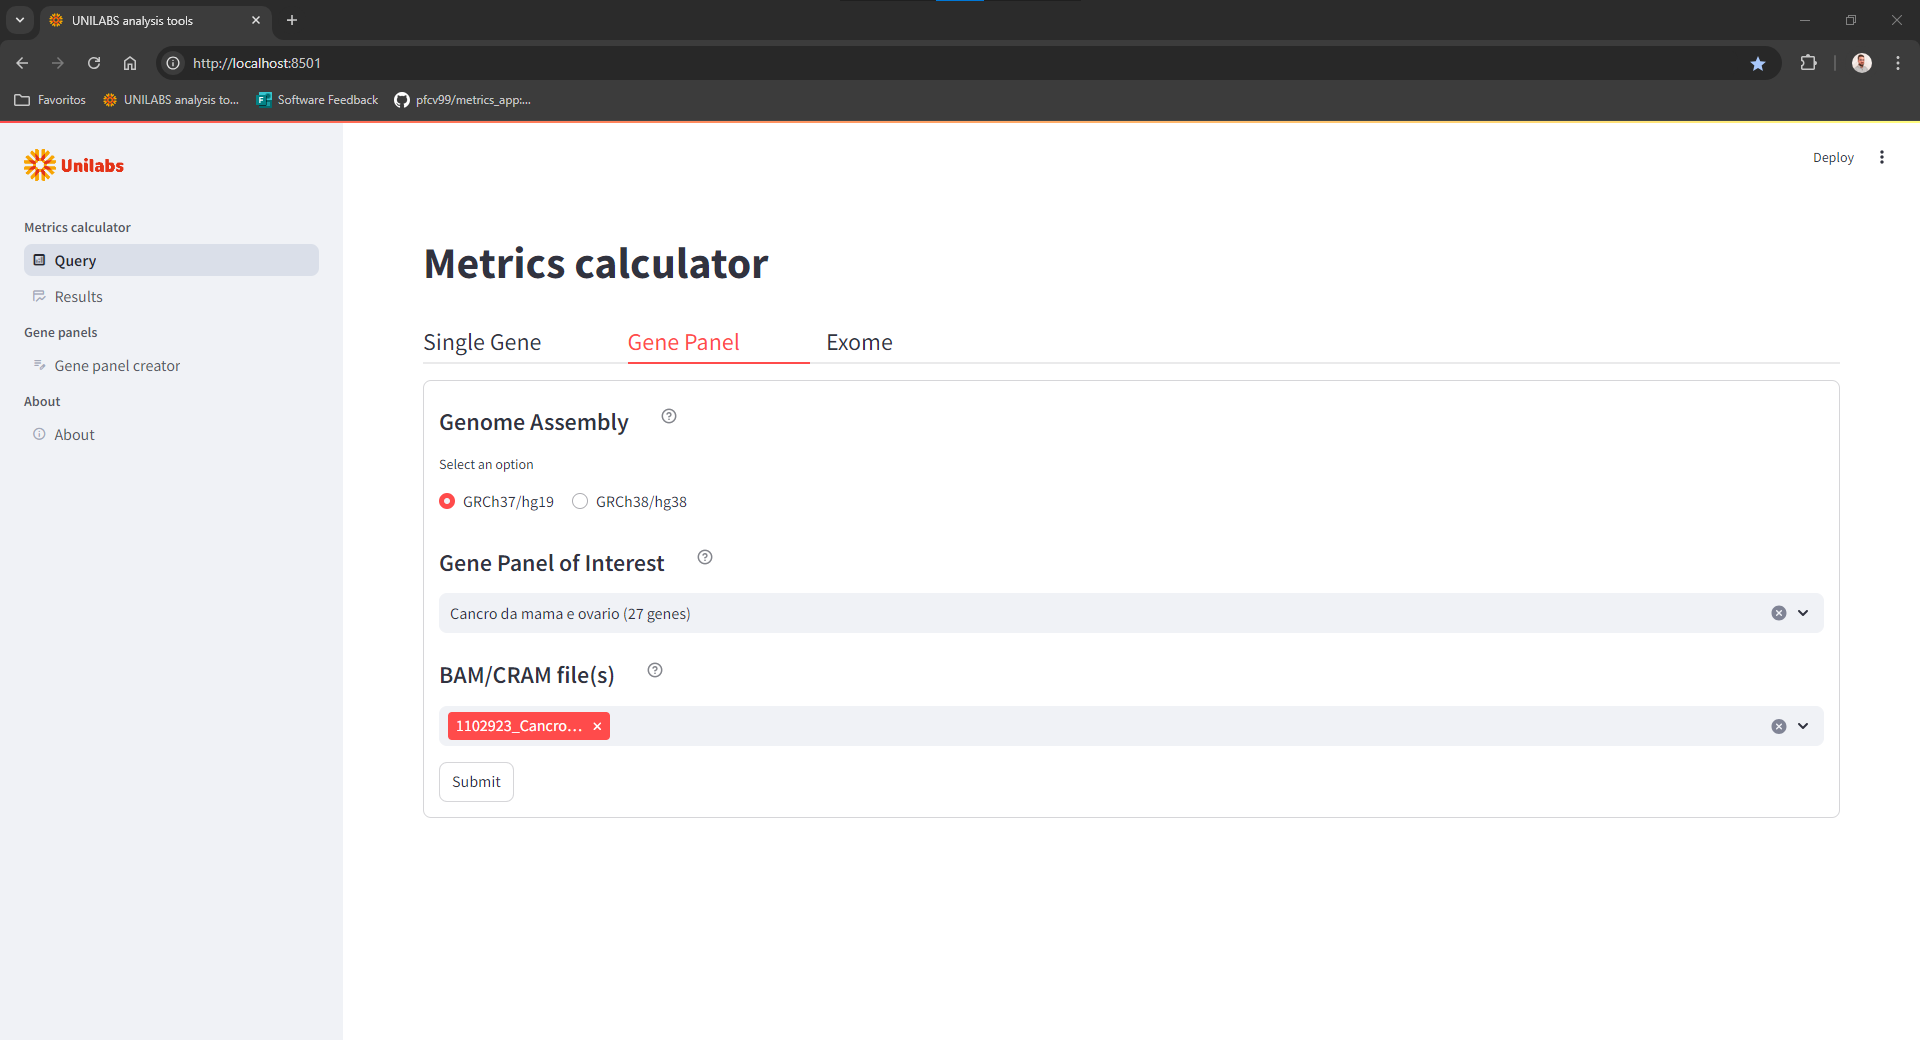
\includegraphics[width=\textwidth]{figs/v3.8.png}
    \caption{Gene Panel Input Selection and Submission}
    \label{fig:panel_input}
\end{figure}

\item \textbf{Overall Results for the Gene Panel}

Once the data is processed, the software generates a comprehensive table of metrics for the entire gene panel. This includes critical metrics such as Size Coding, Size Covered, Breadth of Coverage, and Average Read Depth. These metrics are essential for evaluating the quality of sequencing across all genes in the panel. Figure \ref{fig:panel_results_overall} illustrates the results generated for the gene panel associated with hereditary breast and ovarian cancer. For this specific case, a panel with a Size Coding of 85506 \ac{bp}, the Size Covered was 78360 \ac{bp}, resulting in a Breadth of Coverage of 91.64\%. The Average Read Depth across the panel was 284.9x, with a Minimum Read Depth of 1x and a Maximum Read Depth of 631x. The Depth of Coverage across different thresholds revealed that the panel achieved a Depth of Coverage between 95.7\% and 100\% at the 1x, 10x and 15x, 20x, 30x, 50x and 100x threshold. For the 500x threshold, the Depth of Coverage percentage dropped to 1.9\%, indicating regions less covered by sequencing. 

\begin{figure}[H]
    \centering
    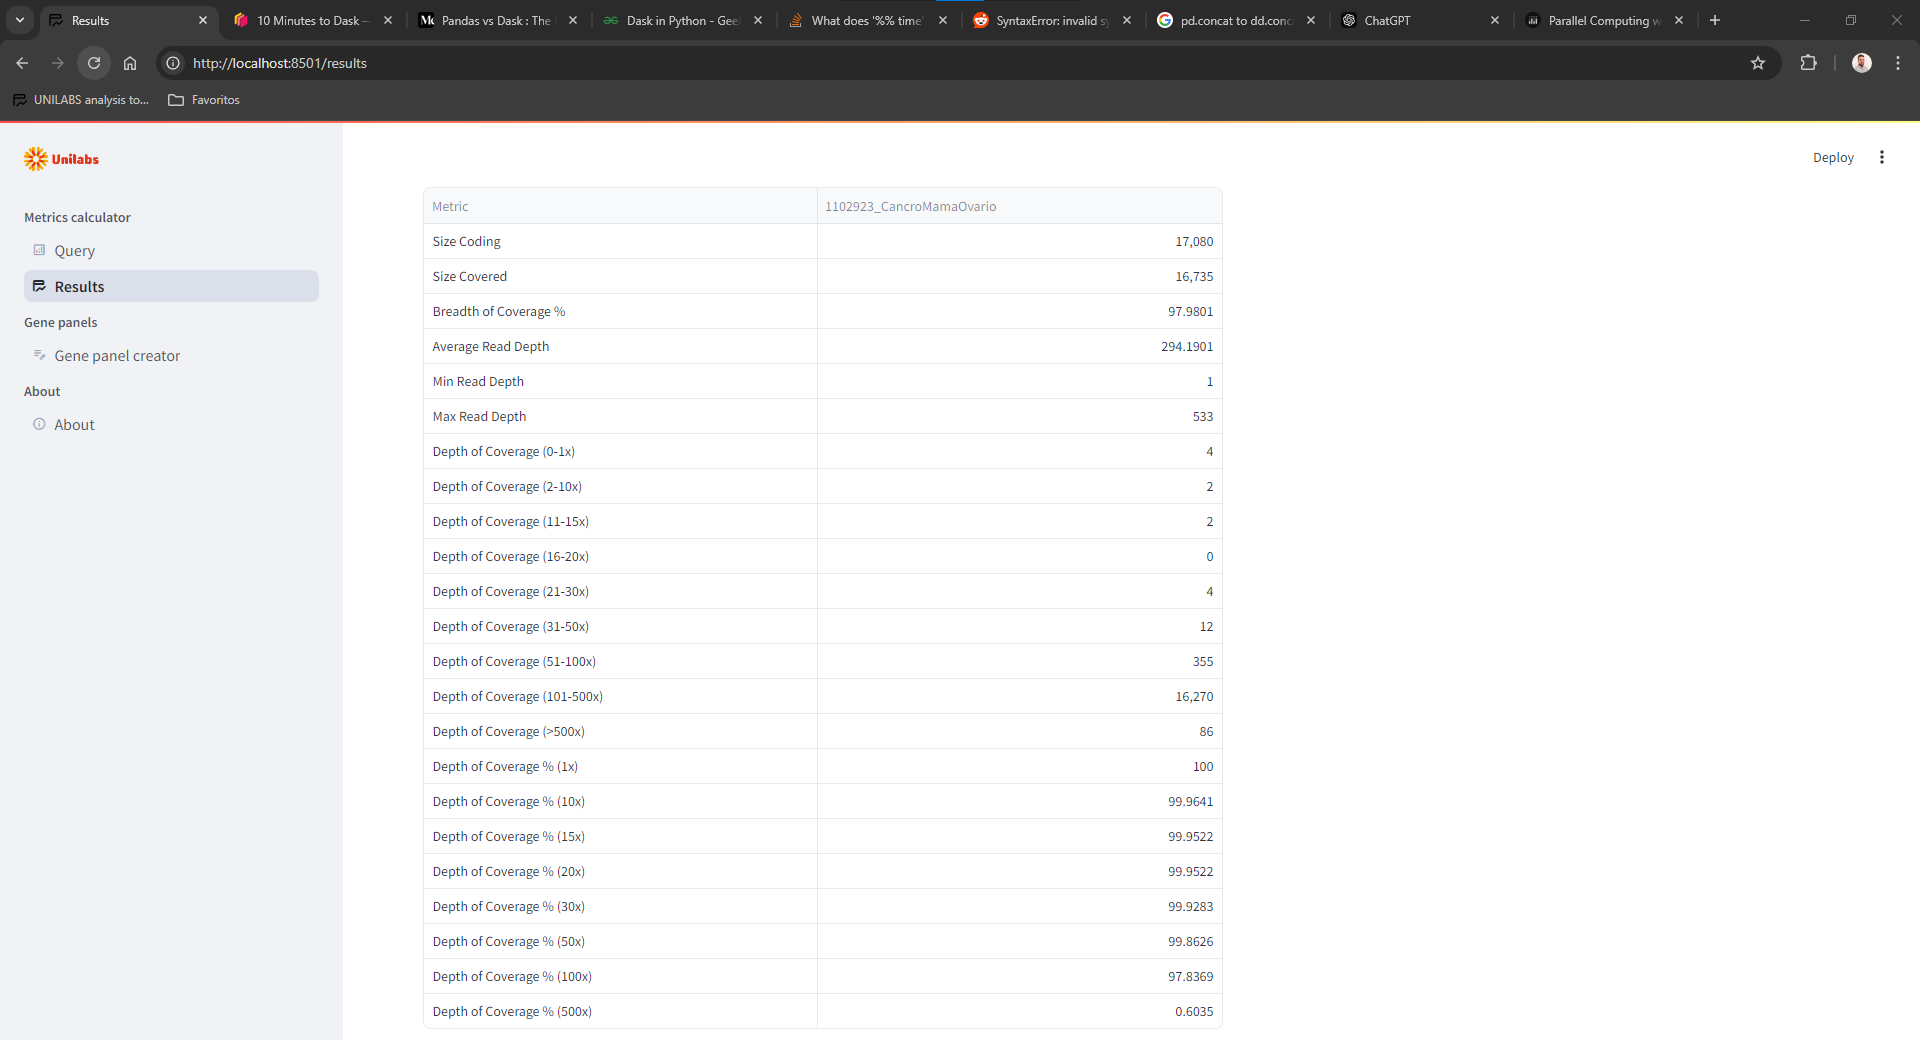
\includegraphics[width=\textwidth]{figs/v3.9.png}
    \caption{Overall Gene Panel Results for Hereditary Breast and Ovarian Cancer}
    \label{fig:panel_results_overall}
\end{figure}

\item \textbf{Individual Gene Metrics}

The software allows users to dive deeper into the metrics for individual genes within the panel. Figure \ref{fig:brca1_results} displays the results for the BRCA1 gene. The Size Coding of BRCA1 was 6343 \ac{bp}, with a Size Covered of 6124 \ac{bp}, resulting in a Breadth of Coverage of 96.5\%. The Average Read Depth for BRCA1 was 345.3x, with a Minimum Read Depth of 1x and a Maximum Read Depth of 533x. The Depth of Coverage across different thresholds showed consistent percentages above 99\% for the 1x, 10x,, 15x, 20x, 30x, 50x and 100x thresholds, with a slight drop to 1.6\% at the 500x threshold.

\begin{figure}[H]
    \centering
    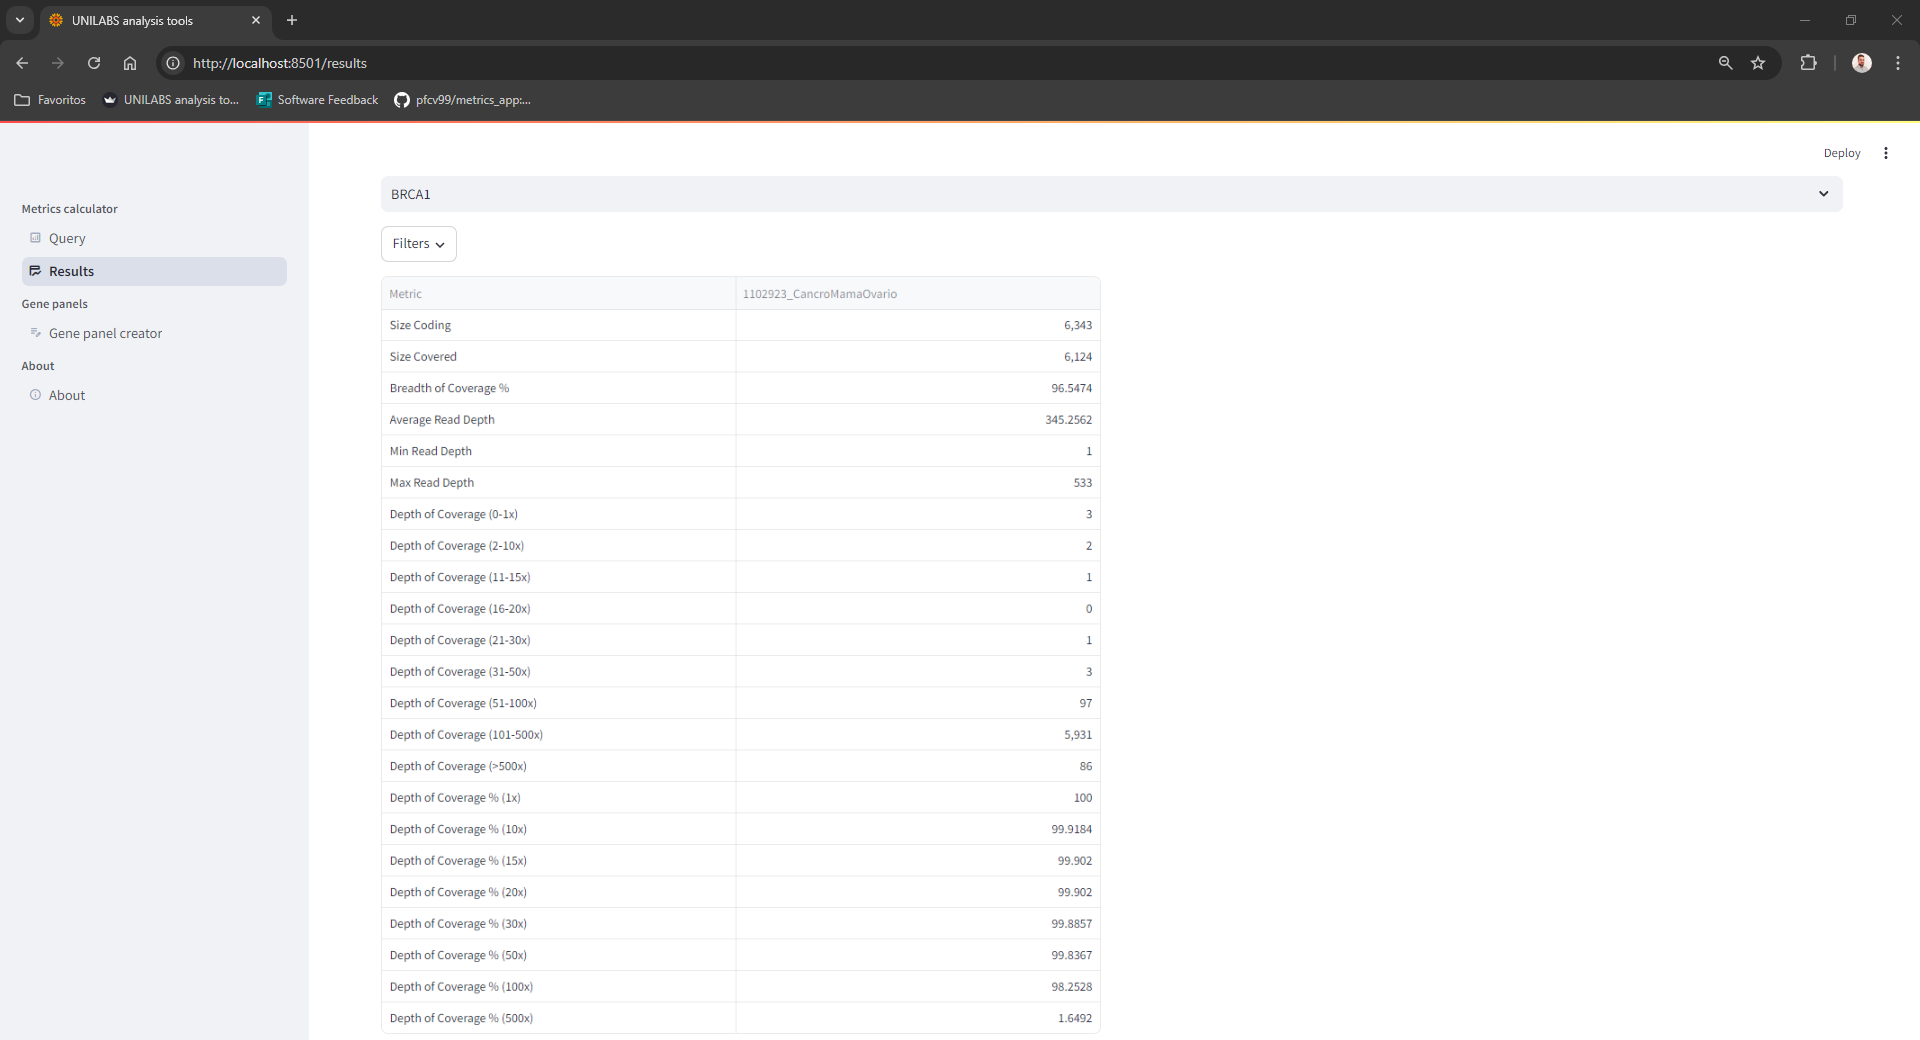
\includegraphics[width=\textwidth]{figs/v3.10.png}
    \caption{Detailed Metrics for the BRCA1 Gene}
    \label{fig:brca1_results}
\end{figure}

\item \textbf{Exon-Level Analysis}

In addition to gene-level metrics, the software also offers exon-level analysis. Users can select specific exons within the genes to obtain a more granular view of the sequencing Depth of Coverage. This level of detail is particularly useful when assessing the completeness of the sequencing across critical regions within each gene. Figure \ref{fig:exon_results} shows the results for the 124th exon of the BRCA1 gene, where key metrics are also displayed. This exon-level detail allows researchers to pinpoint regions that may require additional sequencing or validation. For the 124th exon of BRCA1, the Size Coding was 3532 \ac{bp}, with a Size Covered of 3532 \ac{bp}, resulting in a Breadth of Coverage of 100\%. The Average Read Depth for this exon was 396.5x, with a Minimum Read Depth of 87x and a Maximum Read Depth of 533x. The Depth of Coverage across different thresholds showed consistent coverage percentages of 100\% for the 1x, 10x, 15x, 20x, 30x amd 50x thresholds, with a slight drop to 99.1\% at the 100x threshold. In the 500x threshold, the coverage percentage dropped to 2.9\%.

\begin{figure}[H]
    \centering
    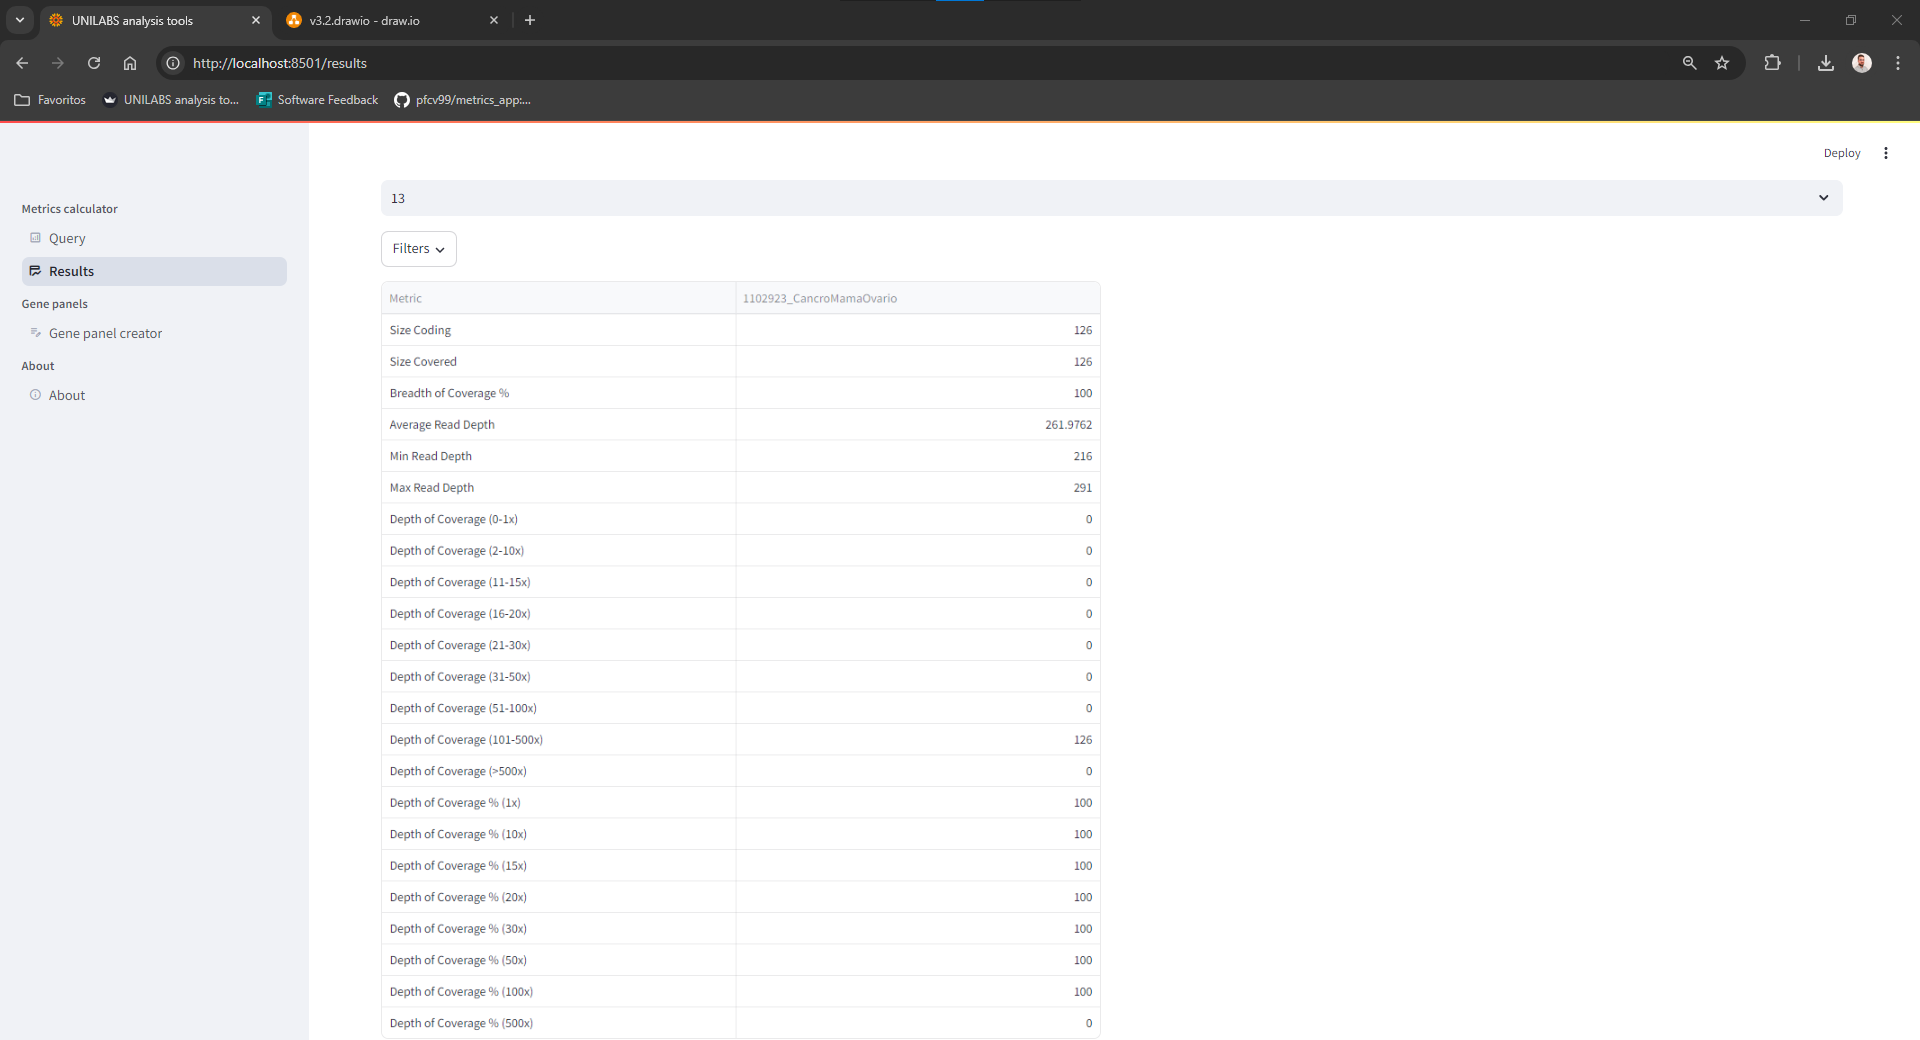
\includegraphics[width=\textwidth]{figs/v3.12.png}
    \caption{Exon-Level Metrics for the BRCA1 Gene}
    \label{fig:exon_results}
\end{figure}

The gene panel analysis feature provides a powerful tool for evaluating sequencing coverage across multiple genes simultaneously. By offering both gene-level and exon-level insights, the software ensures that researchers can thoroughly assess the quality of their sequencing data, identify potential gaps in coverage, and make informed decisions regarding further analysis or re-sequencing.

\end{itemize}

\section{Test and Validation}

To validate the tool, each \ac{bam} file was analyzed using the commercial software Omnomics, and the results were compared with those obtained from the developed software. The analyses were performed separately for a Single Gene and a Gene Panel, ensuring that each \ac{bam} file was used for its respective analysis.

\subsection{Single Gene Analysis}

The gene TP53 was selected for the Single Gene analysis, and the results obtained from the developed software were compared with those from Omnomics. The metrics compared included Average Read Depth and Depth of Coverage \% (1x, 10x, 20x, 30x, 50x, 100x, 500x).

\begin{table}[]
    \centering
    \caption{Comparison of Metrics between Unilabs Software and Omnomics for Gene TP53}
    \label{tab:omnomicsVSunilabs}
    \begin{tabular}{lrr}
    \textbf{Metric}                      & \textbf{Unilabs Software} & \textbf{Omnomics} \\
    \hline
    Average Read Depth          & 757.20           & 891      \\
    Depth of Coverage \% (1x)   & 100              & 100      \\
    Depth of Coverage \% (10x)  & 100              & 100      \\
    Depth of Coverage \% (20x)  & 100              & 100      \\
    Depth of Coverage \% (30x)  & 100              & 100      \\
    Depth of Coverage \% (50x)  & 100              & 100      \\
    Depth of Coverage \% (100x) & 99.92            & 99.90     \\
    Depth of Coverage \% (500x) & 52.76            & 59      
    \end{tabular}
\end{table}

The comparison of the results between the two software solutions highlights some significant differences. The most notable is in the "Average Read Depth" metric, where the developed software reported an average depth of 757.20, while Omnomics recorded a higher value of 891. This discrepancy is largely attributed to the differences in the reference \ac{bed} files used by each tool. The developed software utilizes an optimized \ac{bed} file from MANE, whereas Omnomics employs a UCSC Genes \ac{bed} created using the Table Browser tool from the Genome Browser, specifically targeting the TP53 gene and extending it by 8 \ac{bp}. These differences in \ac{bed} files lead to variations in the regions covered, directly impacting metrics like Average Read Depth.

Both tools reported identical results for the Depth of Coverage \% across lower thresholds, such as 1x, 10x, 20x, 30x, and 50x, indicating full coverage for those depths. However, slight deviations emerge at higher coverage thresholds. For example, the Depth of Coverage \% (100x) shows almost identical values, with Unilabs Software reporting 99.92\% and Omnomics reporting 99.9\%.

The Depth of Coverage \% (500x) shows a more noticeable difference, with Unilabs Software reporting 52.76\%, while Omnomics reported 59\%. This deviation could be explained once again by the different regions covered by the respective \ac{bed} files, which affects the depth distribution across the regions analyzed.

While both tools offer highly accurate coverage analyses, the variations in metrics such as Average Read Depth and higher coverage percentages reflect differences in the underlying reference files. The developed software's use of the MANE based \ac{bed} and Omnomics reliance on the UCSC Genes \ac{bed} result in slight but consistent differences, especially in metrics sensitive to the exact regions analyzed.

\subsection{Gene Panel Analysis}

For the analysis of a gene panel the previous panel "Cancro da mama e ovário (27 genes)" was used. One of the \ac{bam} files used was compared between the Unilabs Software and the commercial tool Omnomics. The results are detailed in Table \ref{tab:panel_omnomicsVSunilabs}, highlighting the differences between the two tools for several metrics.

\begin{table}[]
\centering
\caption{Comparison of Metrics between Unilabs Software and Omnomics for Gene Panel: Cancro da mama e ovário (27 genes)}
\label{tab:panel_omnomicsVSunilabs}
\begin{tabular}{lrr}
\textbf{Metric}                      & \textbf{Unilabs Software} & \textbf{Omnomics} \\ \hline
Average Read Depth          & 284.90           & 388      \\
Depth of Coverage \% (1x)   & 100              & 99.60     \\
Depth of Coverage \% (10x)  & 99.26            & 99.50     \\
Depth of Coverage \% (20x)  & 98.96            & 99.40     \\
Depth of Coverage \% (30x)  & 98.87            & 99.20     \\
Depth of Coverage \% (50x)  & 98.39            & 98.80     \\
Depth of Coverage \% (100x) & 95.70            & 96.10     \\
Depth of Coverage \% (500x) & 1.90             & 27.60    
\end{tabular}
\end{table}

The comparison between Unilabs Software and Omnomics for this gene panel reveals several key differences in the reported metrics. Most notably, the Average Read Depth shows a significant disparity, with Unilabs Software reporting a depth of 284.9, while Omnomics reports a substantially higher value of 388. This difference can once again be attributed to the different \ac{bed} files used by each tool.

For the Depth of Coverage \% metrics, both tools report similar values, though some minor differences are present. At the 1x coverage threshold, Unilabs Software reports 100\%, while Omnomics reports 99.6\%. Similarly, for the 10x, 20x, 30x, and 50x thresholds, the differences remain small, with Omnomics consistently reporting slightly higher percentages. However, at the 100x threshold, the tools report nearly identical values, with Unilabs Software at 95.70\% and Omnomics at 96.1\%.

The most significant divergence occurs at the 500x threshold. Unilabs Software reports a very low value of 1.90\%, while Omnomics reports a much higher 27.6\%. This discrepancy is likely due to the differing regions targeted by the \ac{bed} files, with Omnomics potentially including regions of higher coverage within the panel that are not present in the Twist \ac{bed} file used by Unilabs Software.

Overall, the comparison between the two tools highlights the importance of the reference \ac{bed} file used in determining coverage metrics. While the results are largely consistent across most coverage thresholds, notable differences, particularly in the Average Read Depth and the highest coverage levels, underscore the impact of \ac{bed} file selection on the analysis results.

\section{Performance}


\section{Users feedback}

In order to evaluate the usability and effectiveness of the developed software, a feedback questionnaire was designed and distributed to a group of 14 users from Unilabs Genetics team with diverse professional backgrounds. The primary objective of this questionnaire was to gather insights into the user experience, performance, and overall satisfaction with the software. Given that the software was intended to cater to a wide range of technical expertise, from laboratory technicians to bioinformatics specialists, it was crucial to ensure that it met the functional and usability needs of these varied audiences.

The questionnaire consisted of multiple sections aimed at assessing specific aspects of the software, including the ease of navigation, clarity of the interface, speed of performance, and the usefulness of the analytical metrics provided. Participants were asked to rate their experience on a numerical scale while also providing qualitative feedback on areas where the software excelled or required improvement.

In addition to rating the software's technical performance, respondents were encouraged to share their thoughts on the software's design, user interface, and the clarity of instructions provided throughout the analysis process. This approach allowed for a comprehensive evaluation that encompassed both the functional and aesthetic dimensions of the user experience. The ultimate goal of this survey was to identify key areas that could be optimized to further align the software with the needs of its users, while also validating its current performance and utility in the field of genomic analysis.

Overall, the feedback was overwhelmingly positive. Most users reported a high level of satisfaction with the software's intuitive interface, with many describing it as "very intuitive" and "user-friendly." All respondents confirmed that they did not experience any difficulties navigating the software. Additionally, the explanations provided for the functionalities were considered clear by all users, indicating that the design and guidance within the software successfully facilitated a smooth user experience.

In terms of performance, the software was well-regarded for its speed and efficiency. The majority of users rated the software's performance highly (considering the test dataset), with ratings ranging from 3 to 5 on a scale of 1 to 5, with 5 representing the fastest performance. The respondents also praised the ease with which they could input data and obtain analysis results, with all participants stating that the process was straightforward. This indicates that the software effectively supports the users workflow, minimizing potential barriers to data input and result interpretation.

The analysis results themselves were deemed clear and comprehensible, with users unanimously agreeing that the software met or exceeded their expectations. Notably, the metrics provided by the software were highlighted as particularly useful for their work, suggesting that the software successfully addresses key analytical needs in genomic analysis. Users expressed a high likelihood of recommending the software to colleagues, demonstrating strong approval of its functionality and usefulness.

Suggestions for improvement were minimal, with a few users recommending performance enhancements and the inclusion of additional features, such as tailoring the software for \ac{cnvs} analysis. Nevertheless, users appreciated the versatility of the software, particularly the ability to zoom into specific regions and generate metrics for gene panels, genes and exons.

The feedback from the questionnaire indicates that the software is well-received, providing a user-friendly, intuitive, and efficient tool that meets the needs of various professionals in the genomic field. The overwhelmingly positive responses suggest that the software has significant potential for widespread adoption, with only minor adjustments needed to further enhance its performance and expand its capabilities.




